\section*{Übung 9}
\subsection*{Aufgabe 1}
\subsubsection*{Lösungsidee}
Bei dieser Aufgabe wird eine doppelt verkettete Liste, die eine einfach verkettete Liste enthält, initialisiert. Die Liste wird am Anfang auf Nil gesetzt. Alles weitere wird in der appendToAmazonList behandelt. Falls die Liste Nil ist, wird ein neues Element für diese Liste erstellt. Bei jedem einlesen einer Text Zeile wird überprüft ob die Zeile den Namen oder den Wunsch eines Kindes enthält. Der Name und der Wunsch wird dem appendToAmazonList übergeben. Falls ein Wunsch bereits enthalten ist, wird der Name zur Wishers Liste hinzugefügt. Andernfalls wird ein neues Element erstellt mit dem Namen des Kindes als Wisher. 
\newline

\lstinputlisting[language=Pascal] {../XmasWish.pas}
\begin{figure}[H]
	\centering
	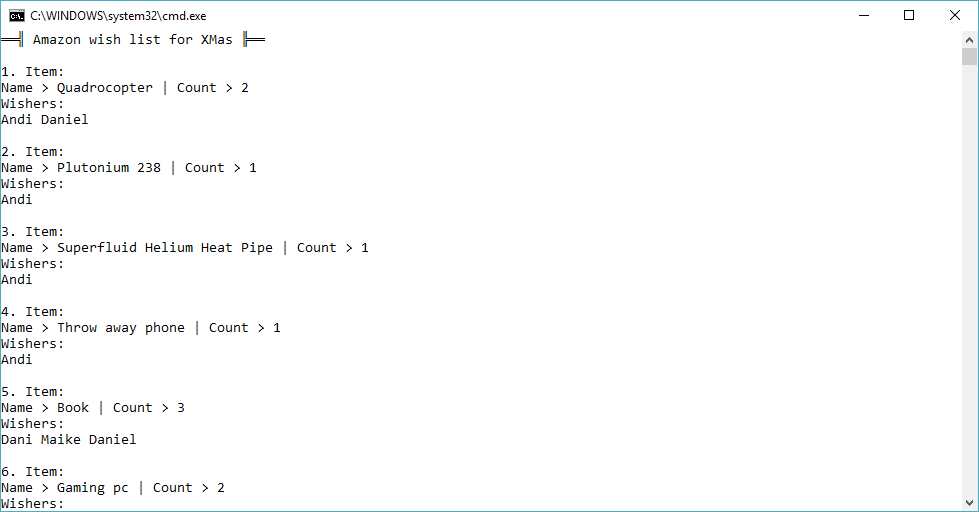
\includegraphics[scale=0.65]{./pictures/XmasWish.png}
	\caption{Testfälle XmasWish 1}
	\label{fig: XmasWish1}
\end{figure}

\begin{figure}[H]
	\centering
	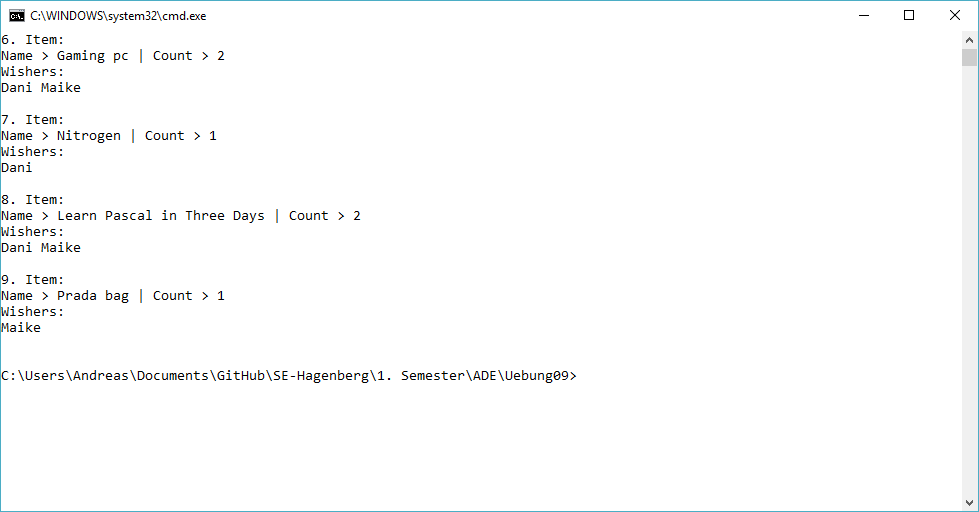
\includegraphics[scale=0.65]{./pictures/XmasWish_2.png}
	\caption{Testfälle XmasWish 2}
	\label{fig: XmasWish2}
\end{figure}

\lstinputlisting[language=C] {../Wishes.txt}

\section*{Testfälle}
Eine Liste wird erstellt und ausgegeben. Die Liste wird mithilfe der Wishes.txt erstellt.
Zu sehen ist ein Element der Liste und die Namen der Kinder die sich dasselbe wünschen.
\newpage
\subsection*{Aufgabe 2}
\subsubsection*{Lösungsidee}
Für diese Aufgabe wird sowohl eine Rekursive sowie eine Iterative Funktion erstellt. Bei einem Rekursiven Aufruf wird die Funktion immer wieder aufgerufen bis ein Punkt erreicht bzw. eine Bedingung erfüllt ist an der der erneute Funktionsaufruf nicht mehr ausgeführt wird. Für die Berechnung wird durch beobachten der Beispiele eine mathematische Funktion erstellt. Diese lautet: 3$^{h-1}$ wobei h die Höhe darstellt.
\newline

\lstinputlisting[language=Pascal] {../CandleonTree.pas}
\begin{figure}[H]
	\centering
	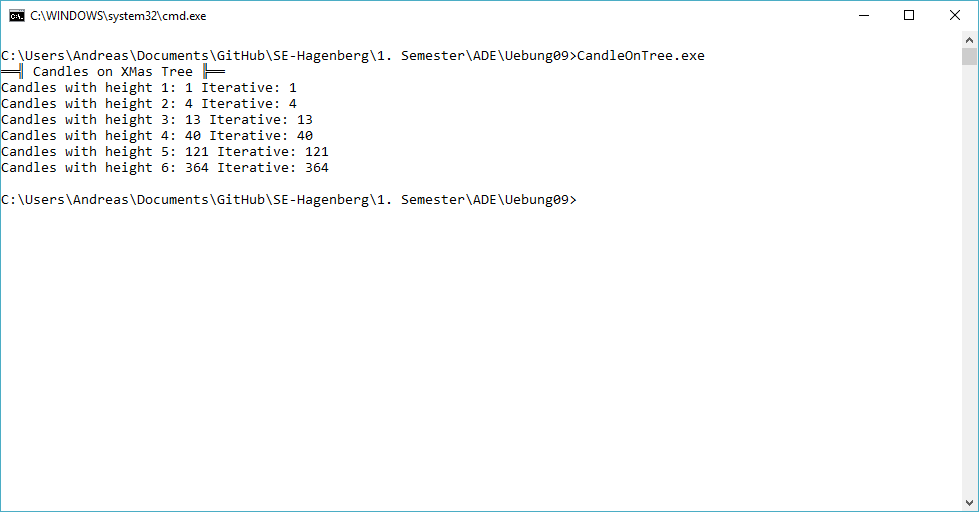
\includegraphics[scale=0.65]{./pictures/CandlesOnTree.png}
	\caption{Testfälle CandleonTree}
	\label{fig: CandleonTree}
\end{figure}

\section*{Testfälle}
Die Testfälle zeigen die Kerzenanzahl bei entsprechender Höhe des Baumes mit der iterativen und der rekursiven Funktion.
\newpage

\subsection*{Aufgabe 3}
\subsubsection*{Lösungsidee}
Bei dieser Aufgabe muss wie bei der vorherigen Aufgabe die mathematische Funktion ermittelt werden. Zusätzlich wird auch überprüft ob das eingegebene Wort ungerade und nicht 0 ist. Da bei jedem Wort das länger als 3 ist drei Wege gibt bei denen es keine Abzweigungen gibt, wird der Zähler um 3 erhöht. Danach wird der counter entsprechend mit (Länge Worte - 3)*2 erhöht. Das wird solange durchgeführt bis die Länge < 3 und die Abbruchbedingung erfüllt ist.
\newline

\lstinputlisting[language=Pascal] {../XmasFire.pas}
\begin{figure}[H]
	\centering
	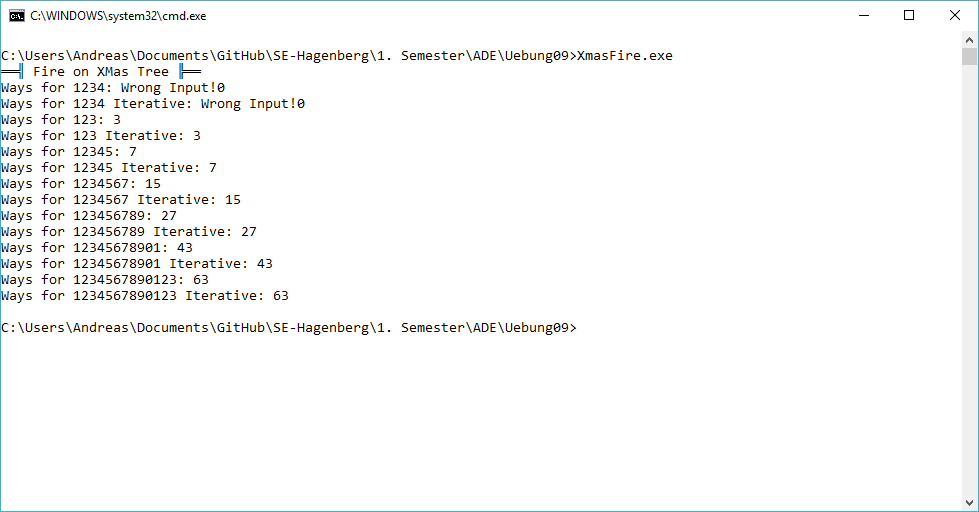
\includegraphics[scale=0.65]{./pictures/XmasFire.png}
	\caption{Testfälle XmasFire}
	\label{fig: XmasFire}
\end{figure}

\section*{Testfälle}
Die Testfälle zeigen Anzahl der möglichen Wege für das jeweilige Wort.
\newpage



